\documentclass[11pt,a4paper]{article}
\usepackage[left=2cm,text={17cm,25cm},top=2.5cm]{geometry}
\usepackage[T1]{fontenc}
\usepackage[english]{babel}
\usepackage[utf8]{inputenc}
\usepackage{url}
\usepackage{graphicx}
\usepackage{pdfpages}
\usepackage[colorinlistoftodos,prependcaption,textsize=tiny]{todonotes}

\graphicspath{ {figs/} }

\begin{document}

\begin{center}
	\LARGE{SIN -- Inteligentní systémy}\\
	\Large{Implementace meteostanice s autonomním řízením}
	\vspace{0.5cm}

    \begin{centering}
        \small{Bc. Petr Stehlík <xstehl14@stud.fit.vutbr.cz>}
    \end{centering}

    \begin{centering}
        \small{Bc. Matej Vido <xvidom00@stud.fit.vutbr.cz>}
    \end{centering}

	\vspace{0.2cm}

\end{center}

\section{Úvod}
Cílem projektu je navrhnout a implementovat meteostanici využívající MQTT protokol pro zasílání naměřených hodnot serveru. Server implementuje databázi a webové grafické uživatelské rozhraní (GUI), analyzuje historické hodnoty a na jejich základě řídí akce aktuátorů.

Meteostanice měří teplotu, vlhkost a tlak vzduchu; vlhkost v květináči a světelnou intenzitu. Navržené aktuátory jsou ovládání žaluzií, klimatizace, topení a zavlažování rostlin. Vše je autonomně ovládáno na základě předem stanovených pravidel.

GUI zobrazuje aktuální a historické naměřené hodnoty jednotlivých senzorů, trendy a naposledy vykonané akce aktuátorů společně s krátkodobou předpovědí počasí získanou z volně dostupných zdrojů.

\section{Nástroje pro monitoring a řízení}
Na trhu je velké množství dostupných nástrojů pro monitoring a řízení a to i na poli chytrých domácností. Je zde mnoho komerčních a uzavřených systémů pro automatizaci domácnosti. V současnosti nejznámější a pravděpodobně i nejrozšířenější je Apple Home\footnote{\url{https://www.apple.com/lae/ios/home/}}, který využívá protokolu Homekit také od společnosti Apple. Na trhu existuje pro Apple Home velké množství produktů a neustále se jejich počet zvyšuje. Existuje ale i mnoho open-source nástrojů pro řízení domácnosti. Jejich nejrozšířenější zastupitele jsou zde v krátkosti popsány.

\subsection{Grafana}
Grafana\footnote{\url{https://grafana.com/}} je vizualizační a analytický nástroj pro data zachycená v čase. Grafana samotná není primárně určena pro monitoring a řízení chytrých domácností, ale je natolik upravitelná, že existují konfigurace, které toto užití zpřístupňují. Je dostupná s mnoha rozšířeními a zdroji dat. Uživatel si vytvoří dashboard, který si následně nakonfiguruje a seskládá z dostupných modulů. Tyto moduly mimo dalších funkcionalit umožňují zobrazit čárový graf, jednotlivé hodnoty, trendy hodnot a s pomocí modulů i různé přepínače.

\subsection{Domoticz}
Domoticz\footnote{\url{https://domoticz.com/}} je kompletním open-source systémem pro domácí automatizaci. Tento nástroj dovoluje monitorovat, řídit a konfigurovat mnoho různých zařízení od různých výrobců. Disponuje i automatickým učením senzorů a aktuátorů. Rozhraní pro uživatele je vytvořeno jako webová stránka dostupná na stroji s lokální instalací Domoticz.

\subsection{OpenHAB}
OpenHAB\footnote{\url{https://www.openhab.org/}} je dalším velmi známým zástupcem open-source nástrojem pro domácí automatizaci. Podporuje velké množství platforem, výrobců a zařízení. Dokáže integrovat mnoho systémů do jednoho centrálního řešení, které lze ovládat mobilní aplikací, webových rozhraním nebo nativní desktopovou aplikací. Pro automatizaci disponuje rozsáhlým systémem pro tvorbu komplexních pravidel.

\subsection{Home Assistant}
Home Assistant\footnote{\url{https://home-assistant.io/}} je primárně navrhován pro užívání na Raspberry Pi. Jako předchozí nástroje také podporuje široké množství výrobců a zařízení. Také disponuje konfigurovatelným webových rozhraním s přehledy zařízení a kontrolou aktuátorů.

\subsection{BeeeOn}
BeeeOn\footnote{\url{https://beeeon.org/wiki/Main\_Page}} je systém pro domácí automatizaci vyvíjený na FIT VUT v Brně. Tento systém je primárně vyvíjen jako bezpečná domácí brána pro různé IoT zařízení. Oproti předchozím systémům je nutno pro plnou funkcionalitu systému vlastnit domácí bránu, kterou lze propojit s několika výrobci a jejich zařízeními. BeeeOn disponuje Android mobilní aplikací pro ovládání domácnosti a prototypem webového rozhraní.

\subsection{Vlastní řešení}
%TODO do cestiny
Okrem uvedených kompletných riešení pre monitoring a analýzu riadiachich systémov je možné poskladať vlastné riešenie
z dostupných open-source knižníc, frameworkov a nástrojov.

Rozšíreným frameworkom pre tvorbu klientskej časti webových aplikácií je Angular\footnote{\url{https://angular.io/}}.
Angular napísaný v jazyku TypeScript umožňuje jednoduchú integráciu rôznych knižníc pre zobrazovanie grafov a tvorbu dashboardov.

K implementácii serverovej časti webovej aplikácie je možné použiť framework Flask\footnote{\url{http://flask.pocoo.org/}} v jazyku Python.
Flask umožňuje rýchlu a jednoduchú tvorbu REST API na prepojenie serverovej a klientskej časti webovej aplikácie.
Výhodou použitia jazyku Python pre tvorbu serverovej časti aplikácie je, že obsahuje moduly pre obsluhu databázového systému
a zabezpečenie sieťovej komunikácie s ďalšími prvkami celého riadiaceho systému.

Mosquitto\footnote{\url{https://mosquitto.org/}} je voľne dostupný broker pre MQTT protokol používaný v prostredí systémov IoT podporujúci rôzne platformy.

\section{Architektura a implementace}
\subsection{Hardware}
Základem pro hardware byly zvoleny Raspberry Pi 2 jako server a Raspberry Pi Zero W jako samotná meteostanice. Server realizován jako Raspberry Pi 2 zpřístupňuje uživateli minimalistické webové rozhraní a slouží jako MQTT broker pro meteostanici. Také jsou zde ukládány všechny naměřené hodnoty do SQLite3 databáze.

K Raspberry Pi Zero W jsou připojeny následující senzory:

\begin{itemize}
    \item DHT11 - digitální senzor pro měření teploty a vlhkosti vzduchu
    \item BMP180 - digitální senzor pro měření barometrického tlaku, teploty a nadmořské výšky
    \item TEMT6000 - analogový senzor pro měření intenzity okolního světla
    \item YL-69 společně s YL-38 - analogový senzor pro měření vlhkosti půdy
\end{itemize}

Pro konverzi analogových senzorů je použit AD převodník MCP3008.


\begin{figure}[htb]
    \centering
    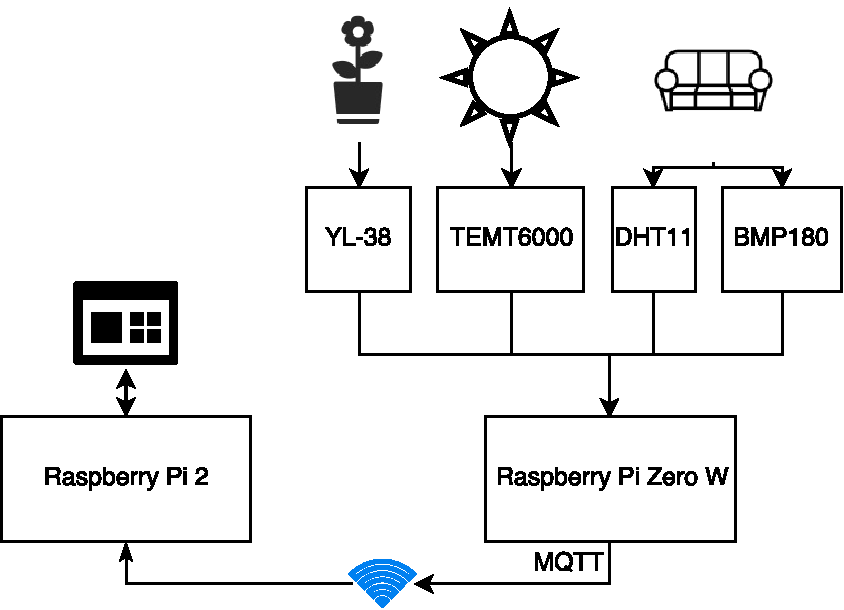
\includegraphics[width=0.5\linewidth]{weather-station-scheme}
    \caption{This is a figure.}
\end{figure}

\todo[inline]{schéma HW zapojení (rpis)}
\todo[inline]{aktuátory}

\subsection{SW}
aktuátory
mqtt (co to je, jak se pouziva) + mosquitto + topic schemes
zapojení dashboardu (fe, be, db, rest api)
popis technologii (angular, flask, sqlite)

\section{Výsledky}
\label{sec:res}

\section{Závěr}
\label{sec:sum}

\end{document}
